%Art des Dokuments%
\documentclass[a4paper, 11pt]{article}

%Packete
\usepackage{ifxetex,ifluatex}
\usepackage{etoolbox}
\usepackage[svgnames]{xcolor}
\usepackage{amssymb}
\usepackage{tikz}
\usepackage{tcolorbox}
\usepackage{framed}
\usepackage[]{algorithm2e}
\usepackage{chngcntr}
\usepackage{amsmath}
\counterwithin*{equation}{section}
\counterwithin*{equation}{subsection}
\newif\ifxetexorluatex
\ifxetex
\xetexorluatextrue
\else
\ifluatex
\xetexorluatextrue
\else
\xetexorluatexfalse
\fi
\fi
\ifxetexorluatex
\usepackage{fontspec}
\usepackage{libertine}
\newfontfamily\quotefont[Ligatures=TeX]{Linux Libertine O}
\else
\usepackage[utf8]{inputenc}
\usepackage[T1]{fontenc}
\usepackage{libertine}
\newcommand*\quotefont{\fontfamily{LinuxLibertineT-LF}}
\fi
\newcommand*\quotesize{60}
\newcommand*{\openquote}
{\tikz[remember picture,overlay,xshift=-4ex,yshift=-2.5ex]
	\node (OQ) {\quotefont\fontsize{\quotesize}{\quotesize}\selectfont``};\kern0pt}
\newcommand*{\closequote}[1]
{\tikz[remember picture,overlay,xshift=4ex,yshift={#1}]
	\node (CQ) {\quotefont\fontsize{\quotesize}{\quotesize}\selectfont''};}
\colorlet{shadecolor}{Azure}
\newcommand*\shadedauthorformat{\emph}
\newcommand*\authoralign[1]{
	\if#1l
	\def\authorfill{}\def\quotefill{\hfill}
	\else
	\if#1r
	\def\authorfill{\hfill}\def\quotefill{}
	\else
	\if#1c
	\gdef\authorfill{\hfill}\def\quotefill{\hfill}
	\else\typeout{Invalid option}
	\fi
	\fi
	\fi}
\newenvironment{shadequote}[2][l]
{\authoralign{#1}
	\ifblank{#2}
	{\def\shadequoteauthor{}\def\yshift{-2ex}\def\quotefill{\hfill}}
	{\def\shadequoteauthor{\par\authorfill\shadedauthorformat{#2}}\def\yshift{2ex}}
	\begin{snugshade}\begin{quote}\openquote}
		{\shadequoteauthor\quotefill\closequote{\yshift}\end{quote}\end{snugshade}}
\usepackage[ngerman]{babel}
\usepackage{color}
\usepackage[a4paper, lmargin={4cm}, rmargin={2cm}, tmargin={2,5cm}, bmargin={2,5cm}]{geometry}
\usepackage{graphicx}
\usepackage{setspace}
\usepackage{framed}
\usepackage{url}
\usepackage{eurosym}
\usepackage{acronym}
\usepackage{listings}
\usepackage{color}
\usepackage{longtable}
\usepackage{courier}
\usepackage[multiple]{footmisc}
\usepackage{selinput}
\usepackage{array}
\usepackage{multirow}
\usepackage{longtable}
\usepackage{amssymb}
\usepackage{booktabs}
\usepackage[framemethod=TikZ]{mdframed}
\newenvironment{theo}[2][]{
	\refstepcounter{theo}
	
\begin{mdframed}[]\relax}{
\end{mdframed}}
\ifstrempty{#1}
{\mdfsetup{
		frametitle={
			\tikz[baseline=(current bounding box.east),outer sep=0pt]
			\node[anchor=east,rectangle,fill=blue!20]
			{\strut Definition~\thetheo};}
	}
}{\mdfsetup{
		frametitle={
			\tikz[baseline=(current bounding box.east),outer sep=0pt]
			\node[anchor=east,rectangle,fill=blue!20]
			{\strut Definition~\thetheo};}
	}
}
\mdfsetup{
	innertopmargin=10pt,linecolor=blue!20,
	linewidth=2pt,topline=true,
	frametitleaboveskip=\dimexpr-\ht\strutbox\relax
}
\newcommand*{\theadtext}[1]{{\tiny #1}}
\newcommand*{\thead}[1]{\multicolumn1{@{}c@{}}{\theadtext{#1}}}
\newcolumntype{C}[1]{>{\centering\arraybackslash\hspace{0pt}}p{#1}}
\newcolumntype{L}[1]{>{\raggedright\arraybackslash\hspace{0pt}}p{#1}}
\newcolumntype{R}[1]{>{\raggedleft\arraybackslash\hspace{0pt}}p{#1}}
\newcounter{pos}
\newcommand*{\pos}{\refstepcounter{pos}\thepos}
\newcommand{\sectionnumbering}[1]{% 
	\setcounter{section}{0}% 
	\renewcommand{\thesection}{\csname #1\endcsname{section}}} 
\newcommand{\Autor}{Tim Saupp}
\newcommand{\MatrikelNummer}{2742603}
\newcommand{\Kursbezeichnung}{TINF15B3}
\newcommand{\FirmenLogoDeckblatt}{\fbox{
\includegraphics[width=3cm]{dhbw-logo}}}
\newcommand{\Was}{Studienarbeit}
\newcommand{\Titel}{Agentenbasierte Modellierung und Simulation schwarmintelligenter Algorithmen am Beispiel der Futtersuche von Ameisen und Bienen}
\newcommand{\AbgabeDatum}{18.05.2018}
\newcommand{\Dauer}{30.10.2017-18.05.2018}
\newcommand{\Abschluss}{Bachelor of Engineering}
\newcommand{\Studiengang}{Informationstechnik}
\newcommand{\BetreuerDHBW}{Prof. Dr. Lausen}
\makeatletter
\newcommand*{\maintoc}{
	\begingroup
	\@fileswfalse
	\renewcommand*{\appendixattoc}{
		\value{tocdepth}=-10000
	}
	\tableofcontents
	\endgroup
}
\newcommand*{\appendixtoc}{
	\begingroup
	\edef\@alltocdepth{\the\value{tocdepth}}
	\setcounter{tocdepth}{-10000}
	\renewcommand*{\contentsname}{
		Verzeichnis der Anh\"ange}
	\renewcommand*{\appendixattoc}{
		\setcounter{tocdepth}{\@alltocdepth}
	}
	\tableofcontents
	\setcounter{tocdepth}{\@alltocdepth}
	\endgroup
}
\newcommand*{\appendixattoc}{
}
\g@addto@macro\appendix{
	\if@openright\cleardoublepage\else\clearpage\fi
	\addtocontents{toc}{\protect\appendixattoc}
}
\makeatother
\clubpenalty = 100
\widowpenalty = 100
\definecolor{dkgreen}{rgb}{0,0.6,0}
\definecolor{gray}{rgb}{0.5,0.5,0.5}
\definecolor{mauve}{rgb}{0.58,0,0.82}
\definecolor{eggshell}{rgb}{0.94, 0.92, 0.84}
\lstset{
	backgroundcolor=\color{eggshell},
	basicstyle=\footnotesize\ttfamily,
	frame=single,
	breaklines=true,	
	commentstyle=\color{dkgreen},
	captionpos=b,
	keywordstyle=\color{blue},
	stringstyle=\color{mauve},
	tabsize=2,
	language=Java,
	numbers=left,
	numbersep=5pt,
	numberstyle=\tiny\color{gray},
	showstringspaces=false}

\addto\captionsngerman{\renewcommand{\abstractname}{Abstract}}




%%%%%%%%%%%%%%%%%%%%%%%%%%%%%%%%%%%%%%%%%%%%%%%%%%%
%Tim Saupp Studienarbeit 2017-2018 5.& 6. Semester%
%%%%%%%%%%%%%%%%%%%%%%%%%%%%%%%%%%%%%%%%%%%%%%%%%%%



\begin{document}
\begin{titlepage}
	\begin{center}
		\vspace*{-2cm}
		\FirmenLogoDeckblatt\hfill
\includegraphics[width=5cm]{logo.jpg}\\[2cm]
		{\Huge \Titel}\\[2cm]
		{\Huge\scshape \Was}\\[2cm]
		{\large für die Prüfung zum}\\[0.5cm]
		{\Large \Abschluss}\\[0.5cm]
		{\large des Studienganges \Studiengang}\\[0.5cm]
		{\large an der}\\[0.5cm]
		{\large Dualen Hochschule Baden-Württemberg Karlsruhe}\\[0.5cm]
		{\large von}\\[0.5cm]
		{\large\bfseries \Autor}\\[1cm]
		{\large Abgabedatum \AbgabeDatum}
		\vfill
	\end{center}
	\begin{tabular}{l@{\hspace{2cm}}l}
		Bearbeitungszeitraum	         & \Dauer 			\\
		Matrikelnummer	                 & \MatrikelNummer		\\
		Kurs			         & \Kursbezeichnung		\\
		Gutachter der Studienakademie	 & \BetreuerDHBW		\\
	\end{tabular}
\end{titlepage}
\newpage
\thispagestyle{empty}
\begin{framed}
	\begin{center}
		\Large\bfseries Erklärung
	\end{center}
	\medskip
	\noindent
	Ich versichere hiermit, dass ich meine \Was\ mit
	dem Titel: {\Titel} selbstständig verfasst und keine anderen als die angegebenen Quellen und
	Hilfsmittel benutzt habe. Ich versichere zudem, dass die eingereichte elektronische Fassung mit der
	gedruckten Fassung übereinstimmt.
	
	\vspace{3cm}
	\noindent
	\underline{\hspace{4cm}}\hfill\underline{\hspace{6cm}}\\
	Ort~~~~~Datum\hfill Unterschrift\hspace{4cm}
\end{framed}
\newpage
\begin{framed}
	\begin{center}
		\Large\bfseries Sperrvermerk
	\end{center}
	\medskip
	\noindent
	Der Inhalt dieser Arbeit darf weder als Ganzes noch in Auszügen Personen
	außerhalb des Prüfungsprozesses und des Evaluationsverfahrens zugänglich gemacht
	werden, sofern keine anders lautende Genehmigung der Ausbildungsstätte vorliegt.
\end{framed}
\newpage
\pagenumbering{Roman}
%Umbenennung Abstract zu Zusammenfassung
\renewcommand{\abstractname}{Zusammenfassung}
\begin{abstract}
\end{abstract}
\newpage
\maintoc           % Inhaltsverzeichnis hier ausgeben%
\newpage
\listoffigures             % Liste der Abbildungen%
\newpage
\listoftables              % Liste der Tabellen%
\newpage
\section*{\Large \textbf Abkürzungsverzeichnis}  
\begin{acronym}[Bash]
	\acro{ABM}{Agentebasierte Modellierung}
	\acro{ACO}{Ameisenkolonieoptimierung}
	\acro{BCO}{Bienenkolonieoptimierung}
	\acro{PSO}{Partikelschwarmoptimierung}
\end{acronym}
\newpage
\pagenumbering{arabic} 
\section{Projektbeschreibung}
\subsection{Motivation}
\subsection{Ziel der Arbeit}
Ziel der Studienarbeit ist die agentenbasierte Modellierung und Simulation der Futtersuche von Ameisen und Bienen. Dazu werden die Strategien der schwarmintelligenten Algorithmen \acs{ACO} und \acs{BCO} auf das Modell der Futtersuche angewandt. Als abstraktes Beispiel wird zudem die \acs{PSO} zum Finden eines globalen Minimums der Rastrigin-Funktion implementiert.
\subsection{Kapitelübersicht}
Kapitel 2 erläutert den Begriff schwarmintelligente Superorganismen, definiert den Begriff Schwarmintelligenz und beschreibt die Grundlagen der agentenbasierte Modellierung. In Kapitel 3 werden die schwarmintelligenten Algorithmen \acs{PSO}, \acs{ACO} und \acs{BCO} vorgestellt. Die implementierten Modelle werden in Kapitel 4 definiert. Zudem wird die Auswahl des verwendeten Frameworks zur Implementierung der definierten Modelle gerechtfertigt. Nachfolgend wird in Kapitel 5 die Implementierung der agentenbasierten Modelle aus Kapitel 4 beschrieben beschrieben.
\newpage
\section{Grundlagen}
\subsection{Schwarmintelligente Superorganismen}
Durch die sensuale Verbindung der Tiere wird die Futtersuche und das Abwehren von Gefahren ohne eine zentrale Lenkung bzw. ohne hierarchische Befehlskette bewältigt. Instinktiv verankerte Regeln sorgen dafür, dass auf bestimmte Aktionen der Tiere in vollkommen deterministischer Weise eine Reaktion erfolgt. Aus dieser dezentralen Interaktion entstehen, bei einem Kollektiv von Tieren, intelligente Resultate auf Makroebene.
\subsubsection{Begriffsdefintion}
Bereits 1911 bezeichnet W. M. Wheeler, amerikanischer Ethologe mit Spezialisierung auf dem Gebiet der Erforschung sozialer Insekten, Kolonien wie die der Bienen und Ameisen als Superorganismen mit emergenten Fähigkeiten\footnote{W.M. Wheeler (1911)}. Abbildung 1 zeigt die Definition und Entstehungsbedingungen kollektiver Intelligenz bei Tierschwärmen:\newline
\begin{figure}[h]
	\begin{center}
	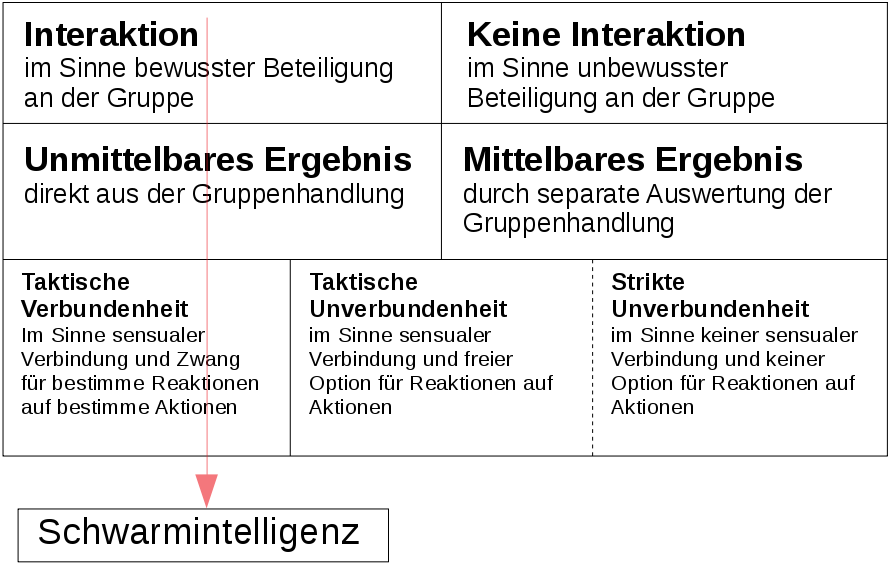
\includegraphics[width=1\textwidth]{schwarmintelligenz}
		\label{defabb}
	\end{center}
	\hspace{1in}\parbox{4in}{\caption[Entstehungsbedingung und Definition kollektiver Intelligenz bei Tierschwärmen]{Entstehungsbedingung und Definition kollektiver Intelligenz bei Tierschwärmen\footnotemark}}
\end{figure}
\footnotetext{A. Aulinger (2013)}
\begin{itemize}
	\item \textbf{Interaktion:} Auf Aktion und Reaktion basierende Interaktion gilt als Grundlage für die Definition des Begriffs Schwarmintelligenz. Anlass dafür ist der in den Tieren vorhandene Überlebensinstinkt, der diese veranlasst, sich bewusst an der Gruppe zu beteiligen.
	\item \textbf{Unmittelbares Ergebnis:} Einzelne Tiere führen Handlungen aus ohne Wissen um das Schwarmergebnis. Das Resultat entsteht unmittelbar aus der Handlung des Schwarms und bedarf keiner externen Aggregation und Auswertung.
	\item \textbf{Taktische Verbundenheit:} Sowohl die sensuale Verbindung der Tiere als auch der in den Tieren verankerte Instinkt zeugen von der taktischen Verbundenheit des Schwarms bestehend aus festen Aktions- und Reaktionsmustern. 
\end{itemize}
\par Zusammenfassend beschreibt der Begriff Schwarmintelligenz ein Phänomen aus dem Tierreich zur Selbstorganisation eines Schwarms, um lebensnotwendige Aufgaben gemeinsam, auf intelligente Weise, zu bewältigen. Dabei vollbringen die Tiere im Schwarm Leistungen, die das Vermögen jedes Einzeltiers übersteigen.
\subsubsection{Ameisen}
Ein Ameisenstaat passt sich ständig an neue Gegebenheiten seiner Umwelt an. Ameisen bilden Staaten mit einigen hundert bis zu mehreren Millionen Individuen. Trotz dieser riesigen Anzahl funktioniert ein Ameisenstaat, da er sich selbst organisiert ohne eine hierarchische Instanz, die einen Überblick über alle Aufgaben besitzt oder diese steuert und verteilt. Stattdessen führen die Handlungen einzelner Ameisen im Zusammenspiel zu einem organisierten Staat, der für die Ameisen sorgt und Nahrung, Brutpflege und Schutz bietet. Interessant sind die Ameisen aufgrund ihrer Fähigkeit effiziente Wege zwischen Futterquellen und dem Ameisenbau ausfindig zu machen\footnote{L. Pintscher (2008)}.
\par Ist der Futtervorrat des Ameisenbaus erschöpft verlassen mehrere Ameisen den Ameisenbau gleichzeitig und begeben sich auf die Futtersuche. Sobald eine Ameise eine Futterquelle gefunden hat, nimmt sie eine Gewichtseinheit des Futters mit und begibt sich auf den Rückweg zum Ameisenbau. Dabei setzt die Ameise Pheromone frei die mit der Zeit verfliegen, um den Weg zur Futterquelle zu markieren. Die Ameise die den kürzesten Weg zu einer Futterquelle gefunden hat legt die Strecke zwischen Ameisenbau und Futterquelle häufiger zurück.  Die Pheromonspur wird durch das häufige Zurücklegen der Strecke intensiviert und dient als sicherer Wegweiser zur Futterquelle. Mitglieder der Kolonie folgen den intensivsten Pheromonspuren. Ist die Futterquelle erschöpft, löst sich die Pheromonspur auf\footnote{R. Wehner (2001)}.
\subsubsection{Bienen}
Um den Gesamtenergiebedarf des Schwarms zu ermitteln, orientiert sich die einzelne Sammlerin an der Wartezeit bei der Übergabe des gesammelten Nektars an die Bienen die den Nektar speichern: Je voller die Futterspeicher, desto länger müssen die Speicherbienen nach leeren Zellen suchen. Je leerer die Speicher, desto schneller wird die Abgabe des Nektars abgewickelt.
\par Im kilometerweiten Gelände besitzt keine Biene den gesamten geographischen Überblick. Sie entscheidet nur lokal über die Rentabilität der Futterquelle. Kundschafterinnen und Sammlerinnen, die von der Futtersuche wiederkehren, führen einen Tanz auf und zeigen unbeschäftigten Bienen damit die Richtung und Entfernung zur gefundenen Futterquelle. Unbeschäftigte Bienen sehen sich die Tänze der im Bienenstock eintreffenden Bienen an und entscheiden sich anschließend für ihr nächstes Ziel. Sobald eine Futterquelle erschöpft ist brauchen die Sammlerinnen länger beim Sammeln und veranlassen aufgrund der geringeren Anzahl an Tänzen weniger Bienen dazu am gleichen Ort zu sammeln.
\newpage
\subsection{Agentenbasierte Modellierung}
Die \ac{ABM} erlaubt eine natürliche Beschreibung von Systemen als eine Sammlung autonomer entscheidungsfähiger Agenten in einer gemeinsamen Umgebung, um emergente Phänomene zu analysieren. Das Ziel der \acs{ABM} besteht darin, durch die Simulation einer Vielzahl an Agenten, das resultierende Systemverhalten zu untersuchen. Nach C. Macal und M. North\footnote{C. Macal, M. North (2010)} verfügt ein agentenbasiertes Modell über folgende Komponenten:
\begin{itemize}
	\item \textbf{Agenten:} Agenten handeln autonom, proaktiv und reaktionär auf der Basis von festgelegten Regeln. Jeder Agent besitzt nur eine eingeschränkte Sicht auf das Gesamtsystem. Sein Wissen über den globalen Zustand des Systems ist immer unvollständig.
	\item \textbf{Agenten-Beziehungen:} Beziehungen zwischen Agenten entstehen durch die proaktive Aktion eines Agenten und die darauffolgende Reaktion eines anderen Agenten oder Interaktionen der Agenten mit der Umgebung.
	\item \textbf{Agenten-Umgebung:} Agenten interagieren innerhalb einer Umgebung mit anderen Agenten und ihrer Umgebung.
\end{itemize}
\subsubsection{Agenten} 
M. Wooldridge und N. Jennings\footnote{M. Wooldridge, N. Jennings (1995)} weisen Agenten die Charaktereigenschaften Autonomie, Proaktivität, Reaktivität und die Fähigkeit zur Interaktion durch Kommunikation zu. Die Handlungsautonomie eines Agenten beschränkt sich auf die Fähigkeit, eigenständig zu entscheiden, welche der ihm zur Verfügung stehenden Aktionen situationsbedingt auszuführen ist. Zielvorgaben bestimmen wann ein Agent welche Aktionen ausführt. Proaktivität beschreibt dabei das zielgerichtete Verhalten eines Agenten der selbst aktiv wird, statt nur auf die Umgebung zu reagieren.\newline
\subsubsection{Agenten-Beziehungen}
Zwischen den Systemelementen bestehen Interaktionsbeziehungen. Die technischen Voraussetzungen für die Kommunikation werden von der Umgebung bereitgestellt. Beziehungen lassen sich einteilen in Interaktion zwischen Agenten und Umgebung, Interaktion zwischen Agenten und organisatorisch bedingte Beziehungen. Die Kommunikation zwischen Agenten kann dabei direkt durch Austausch von Nachrichten oder indirekt über die Veränderung der Umgebung erfolgen.\newline
\subsubsection{Agenten-Umgebung}
Nach S. Russell und P. Norvig\footnote{S. Russel, P. Norvig (2009)} muss eine geeignete Agenten-Umgebung zugänglich, deterministisch, dynamisch, kontrollierbar und teleologisch sein. Eine zugängliche Umgebung erlaubt den Agenten Zugriff auf ihren Zustand. In der Regel beschränkt sich dieser Zugriff jedoch auf den lokalen Wahrnehmungsbereich eines Agenten und erlaubt somit nur Zugriff auf einen Ausschnitt der Umgebung. Deterministisch ist die Umgebung, sobald der Folgezustand vollständig durch den aktuellen Umgebungszustand und die aktuelle Aktion des Agenten bestimmt ist. Kann sich der Zustand der Umgebung durch Aktionen der Agenten ändern, so handelt es sich um eine dynamische und kontrollierbare Umgebung.
\newpage
\section{Schwarmintelligente Algorithmen}
\subsection{Particle Swarm Optimization}
Die klassische \ac{PSO} wurde erstmals im Jahr 1995 von J. Kennedy und R. Ebert beschrieben. Die \acs{PSO} stellt ein, auf der Abfolge von abstrakten Schritten basiertes, Verfahren zur näherungsweisen Lösung von Optimierungsproblemen dar. Zur Lösung des Optimierungsproblems wird eine Population von Partikeln, so lange durch einen Suchraum bewegt, bis eine hinreichende Lösung in einer bestimmten Zeit gefunden wird. Dabei stellt die Position eines Partikels eine potentielle Lösung dar und wird in jedem Zeitschritt neu berechnet\footnote{Y. Liu (2014)}. Um die \acs{PSO} auf ein mathematisches Problem anwenden zu können, müssen zunächst der Suchraum und die Partikel definiert werden\footnote{E. Konstantinos, N. Michael (2010)}.
\subsubsection{Suchraum}
Der Suchraum $S \subset \mathbb{R}^n$ ist ein n-dimensionaler Raum, in dem sich die gesamte Population $X=\{x_{1},x_{2},...,x_{n}\}$ der Partikel bewegt. Damit eine Lösung gefunden werden kann beschränkt sich der Suchraum auf eine endliche Anzahl an möglichen Positionen, die von den Partikeln besucht werden können.
\subsubsection{Partikel}
Jeder Partikel $x_{i}$ besitzt folgende Eigenschaften im Suchraum $S$ zum Zeitpunkt $t$:
\begin{itemize}
	\item \textbf{Position $x_{i}(t)$ im Suchraum $S$ mit einem Funktionswert $f(x_{i}(t))$:} Die aktuelle Position des Partikels $x_{i}$ zum Zeitpunkt $t$ repräsentiert eine potentielle Lösung des Optimierungsproblems. Der dazugehörende Funktionswert $f(x_{i}(t))$ beschreibt die Güte der potentiellen Lösung.
	\item \textbf{Position $x_{b,i}(t)$ im Suchraum $S$ mit einem Funktionswert $f(x_{b,i}(t))$:} Die Position $x_{b,i}$ ist die bisher beste Position des Partikels $x_{i}$ zum Zeitpunkt $t$.
	\item \textbf{Position $x_{g}(t)$ im Suchraum $S$ mit einem Funktionswert $f(x_{g}(t))$:} Die Position $x_{g}$ ist die bisher beste Position des Partikelschwarms zum Zeitpunkt $t$.
	\item \textbf{Geschwindigkeit $v_{i}(t)$:} Die Geschwindkeit $v_{i}$ mit der sich der Partikel durch den Suchraum $S$ zum Zeitpunkt $t$ bewegt.
	\item \textbf{Trägheitskoeffizient $w$:} Der Trägheitskoeffizient $w$ bestimmt die Gewichtung der Geschwindigkeit $v_{i}(t)$ zum Zeitpunkt $t+1$.
	\item \textbf{lokaler Vertrauenskoeffizient $a_{l}$:} Der lokale Vertrauenskoeffizient $a_{l}$ bestimmt die Gewichtung der lokalen Attraktion, bei der Berechnung der Geschwindigkeit $v_{i}(t+1)$.
	\item \textbf{globaler Vertrauenskoeffizient $a_{g}$:} Der globale Vertrauenskoeffizient $a_{g}$ bestimmt die Gewichtung der globalen Attraktion, bei der Berechnung der Geschwindigkeit $v_{i}(t+1)$.
\end{itemize}
Der Trägheitskoeffizient $w$ und die Vertrauenskoeffizienten $a_{l}$ und $a_{g}$ geben an, wie sehr die Partikel sich selbst, ihren eigenen Erfahrungen und den Erfahrungen ihrer Nachbarn vertrauen.
\newpage
\subsubsection{Algorithmus}
\begin{framed}
	\begin{algorithm}[H]
		Initialisiere Partikelschwarm $X$ im Suchraum $S$\;
		\While{Maximale Iterationen nicht erreicht}{
			Bestimme für jeden Partikel Position $x_{i}(t)$\;
			Bestimme für jeden Partikel Geschwindigkeit $v_{i}(t)$\;
			Berechne für jeden Partikel den Funktionswert $f(x_{i}(t))$\;
			\lIf{$f(x_{i}(t))$ besser als $f(x_{b,i}(t))$)}{
				Setze $x_{b,i}(t)$ = $x_{i}(t)$
			}
			\lIf{$f(x_{i}(t))$ besser als $f(x_{g}(t))$}{
				Setze $x_{g}(t))$ = $x_{i}(t)$
			}
			Berechne neue Geschwindigkeit $v_{i}(t+1)$ des Partikels $x_{i}$\;
			Berechne neue Position $x_{i}(t+1)$ des Partikels $x_{i}$\;
		}
		\caption{\acs{PSO} Algorithmus}
		\label{psoalgo}
	\end{algorithm}
\end{framed}
Der abgebildete Algorithmus zeigt den Ablauf der klassischen \acs{PSO}. Im ersten Schritt wird die Population $X$ mit zufälligen Positionen $x_{i}$ im Suchraum $S$ initialisiert. Bis die Anzahl an maximalen Iterationen nicht erreicht ist wird für jeden Partikel geprüft ob der Funktionswert $f(x_{i}(t))$ für die Position $x_{i}(t)$ besser ist als der Funktionswert $f(x_{i}(t-1))$ im vorherigen Schritt an der Position $x_{i}(t-1)$. Ist der Funktionswert $f(x_{i}(t))$ für die Position $x-{i}(t)$ des Partikels besser, wird die bisher beste Position des Partikels $x_{b,i}(t)$ zu $x_{i}(t)$. Zudem wird für jeden Partikel $x_{i}$ geprüft, ob der aktuelle Funktionswert $f(x_{i}(t))$ des Partikels besser ist als der globale Funktionswert $f(x_{g}(t))$. Ist dies der Fall so wird die global beste Position $x_{g}(t)$ zu $x_{i}(t)$.  Für die nächste Iteration wird die Geschwindigkeit $v_{i}(t+1)$ und die neue Position $x_{i}(t+1)$ des Partikels nach folgenden Formeln berechnet:
\begin{equation}
v_{i}(t+1) = wv_{i}(t) + a_{l}r_{1}(x_{b,i}(t) - x_{i}(t)) + a_{g}r_{2}(x_{g}(t) - x_{i}(t))
\end{equation} 
\begin{equation}
x_{i}(t+1) = x_{i}(t) + v_{i}(t+1)
\end{equation}
\par Bei der Berechnung der neuen Geschwindigkeit $v_{i}(t+1)$ wird die Entfernung der Position  $x_{g}(t)$ zur Position $x_{b,i}(t)$ berechnet. Dabei fallen die Zufallszahlen $r_{1}$, $r_{2} \subset \mathbb{R}$ ins Gewicht, sowie die Parameter $w$, $a_{l}$, $a_{g}$, mit denen das Verhalten des Schwarms verändert wird. Gilt $a_{l} > a_{g}$, dann streben die Partikel in Richtung von $x_{b,i}(t)$. Ist $a_{g} > a_{l}$, dann konvergieren die Partikel zur Position $x_{g}(t)$. Abbildung 2 zeigt in grafischer Darstellung die Berechnung der neuen Geschwindigkeit $v_{i}(t+1)$ und der neuen Position $x_{i}(t+1)$.\newline
\begin{figure}[h]
	\begin{center}
		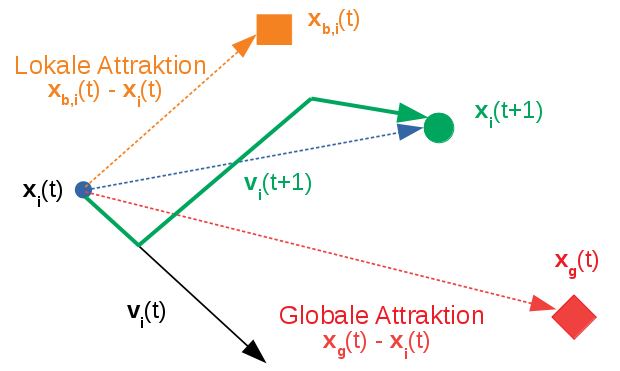
\includegraphics[width=0.50\textwidth]{pso}
	\end{center}
	\hspace{1in}\parbox{4in}{\caption[\acs{PSO}, Berechnung von $x_{i}(t+1)$ und $v_{i}(t+1)$]{Berechnung von $x_{i}(t+1)$ und $v_{i}(t+1)$}}
	\label{psoabb}
\end{figure}
\newpage
\subsection{Ant Colony Optimization}
Die von M. Dorigo\footnote{M. Dorigo (1991)} vorgestellte \ac{ACO} dient, wie die Partikelschwarmoptimierung, der Lösung von Optimierungsproblemen. Zur näherungsweisen Lösung des Optimierungsproblems wird bei der \acs{ACO} eine Population an modellierten Ameisen instanziiert und durch den vom Optimierungsproblem definierten Suchraum bewegt. Die Positionen der modellierten Ameisen repräsentieren potentielle Lösungen des Optimierungsproblems und werden in jedem Zeitschritt neu berechnet. Darüber hinaus ist jede Position im Suchraum mit einem Pheromonniveau markiert. Je höher das jeweilige Pheromonniveau, desto höher ist die Wahrscheinlichkeit, das sich die modellierten Ameisen in Richtung der mit Pheromonen markierten Positionen bewegen.
\subsubsection{Suchraum}
Der Suchraum $S \subset \mathbb{R}^n$ ist ein n-dimensionaler Raum, in dem sich die gesamte Population $X=\{x_{1},x_{2},...,x_{n}\}$ der modellierten Ameisen bewegt. Damit eine Lösung gefunden werden kann beschränkt sich der Suchraum auf eine endliche Anzahl an möglichen Positionen $P=\{p_{1},p_{2},....,p_{n}\}$ die von den modellierten Ameisen besucht werden können. Jeder Position $P$ im Suchraum $S$ ist ein Wert $\tau_{i}$ zugeordnet, der das Pheromonniveau der Position beschreibt.
\subsubsection{Modellierte Ameise}
Jede modellierte Ameise besitzt folgende Eigenschaften im Suchraum $S$ zum Zeitpunkt $t$:
\begin{itemize}
	\item \textbf{Position $x_{i}(t)$ im Suchraum $S$ mit einem Funktionswert $f(x_{i}(t))$:} Die aktuelle Position der modellierten Ameise $x_{i}$ zum Zeitpunkt $t$ repräsentiert eine potentielle Lösung des Optimierungsproblems. Der dazugehörende Funktionswert $f(x_{i}(t))$ beschreibt die Güte der potentiellen Lösung.
	\item \textbf{Position $x_{g}(t)$ im Suchraum $S$ mit einem Funktionswert $f(x_{g}(t))$:} Die Position $x_{g}$ ist die bisher beste Position der Ameisenkolonie zum Zeitpunkt $t$.
	\item \textbf{Teillösungen $C=\{c_{1}(t),c_{2}(t),...,c_{n}(t)\}$ die der modellierten Ameise $x_{i}$ zum Zeitpunkt $t$ zur Verfügung stehen:} Die modellierte Ameise $x_{i}$ wählt aus der ihr zur Verfügung stehenden Teillösungen $C$ zum Zeitpunkt $t$ eine Teillösung. Die gewählte Teillösung entspricht der nächsten Position der modellierten Ameise $x_{i}$ zum Zeitpunkt $t+1$.
	\item \textbf{Wahrscheinlichkeiten $W=\{w_{c_{1}}(t),w_{c_{2}}(t),...,w_{c_{n}}(t)\}$  zur Wahl von $x_{i}(t+1)$:} Die Wahrscheinlichkeiten $W$ werden für die, der modellierten Ameise zur Verfügung stehenden, Teillösungen $C$ berechnet. Die Teillösung mit der höchsten Wahrscheinlichkeit wird von der modellierten Ameise ausgewählt.  	
	\item \textbf{Parameter $\alpha$:} Der Parameter $\alpha$ bestimmt die Gewichtung der Pheromonmarkierungen der Teillösungen $C$ bei der Berechnung der Wahrscheinlichkeiten $W$.
	\item \textbf{Parameter $\beta$:} Der Parameter $\beta$ bestimmt die Gewichtung der Güte der Teillösungen $C$ bei der Berechnung der Wahrscheinlichkeiten $W$
\end{itemize}
Mit $\alpha = 0$ und $\beta = 1$ erhält man einen Greedy-Algorithmus. Umgekehrt erhält man mit $\alpha = 1$ und $\beta = 0$ einen rein zufallsgesteuerten Algorithmus.
\newpage
\subsubsection{Algorithmus}
\begin{framed}
	\begin{algorithm}[H]
		Initialisiere Ameisenkolonie $X$ im Suchraum $S$\;
		\While{Maximale Iterationen nicht erreicht}{
			Berechne für jede modellierte Ameise $x_{i}$ die Wahrscheinlichkeiten $W$ für die möglichen Teillösungen $C$ ausgehend von Position $x_{i}(t)$\;
			Bestimme für jede modellierte Ameise neue Position $x_{i}(t+1)$\;
			\lIf{$f(x_{i}(t+1))$ besser als $f(x_{g}(t))$}{
				Setze $x_{g}(t))$ = $x_{i}(t+1)$
			}
			Berechne für jede gewählte Teillösung die neue Pheromonmarkierung $\tau_{i}(t+1)$ für Position $P$ im Suchraum $S$\;
		}
		\caption{\acs{ACO} Algorithmus}
		\label{acoalgo}
	\end{algorithm}
\end{framed}
Im ersten Schritt des abgebildeten Algorithmus wird die Population $X$ an einer bestimmten Position $P$ im Suchraum $S$ initialisiert. Solange die Anzahl an maximalen Iterationen nicht erreicht ist berechnet jede Ameise die Wahrscheinlichkeiten $W$ für die ihr zur Verfügung stehenden Teillösungen $C$ mit der Formel:
\begin{equation}
W(c_{i}|x_{i}(t)) = \frac{\tau_{c_{i}}^\alpha(t) \cdot [f(c_{i}(t))]^\beta}{\sum_{} c \in C\; \tau_{c}(t)^\alpha \cdot [f(c(t))]^\beta}
\end{equation}
\par Die Wahrscheinlichkeit ist abhängig von dem Pheromonniveau $tau_{c_{i}}$ der jeweiligen Teillösung und der Güte der Teillösung, bestimmt durch $f(c_{i}(t))$. Die Parameter $\alpha$ und $\beta$ verändern das Verhalten der modellierten Ameisen. Gilt $\alpha > \beta$ dann ist das Pheromonniveau der Teillösung ausschlaggebender als die Güte der Teillösung für die Berechnung der Wahrscheinlichkeiten $W$. Sind die Wahrscheinlichkeiten $W$ für alle Teillösungen $C$ berechnet, entscheidet sich die modellierte Ameise für die Teillösung mit der höchsten Wahrscheinlichkeit. Die von der modellierten Ameise gewählte Teillösung entspricht der neuen Position $x_{i}(t+1)$. Im Anschluss wird für jede modellierte Ameise $x_{i}(t)$ geprüft, ob der aktuelle Funktionswert $f(x_{i}(t))$  besser ist als der globale Funktionswert $f(x_{g}(t))$. Ist dies der Fall so wird die global beste Position $x_{g}(t)$ zu $x_{i}(t)$. Am Ende der Iteration werden die Pheromonmarkierungen mit folgender Formel aktualisiert:
\begin{equation}
\tau_{i}(t+1) = (1 - \rho) \tau_{i}(t) + \sum_{x_{i} \in X}\ \Delta \tau_{i}(t)^C
\end{equation}
\par Hierbei ist $\rho$ der konstante Verdunstungsfaktor der Pheromonmarkierungen. Die an der gewählten Teillösung hinterlassene Pheromonmenge $\Delta \tau_{i}(t)^C$ berechnet sich durch die Formel:
\begin{equation}
\Delta \tau_{i}(t)^C = f(c_{i}(t))
\end{equation}
\newpage
\subsection{Bee Colony Optimization}
Die im Zeitraum 1999 bis 2003 von D. Teodorovi\'{c} und P. Lu\u{c}i\'{c} entwickelte \ac{BCO} stellt, wie die \acs{PSO} und \acs{ACO}, ein metaheuristisches Verfahren zur Lösung von Optimierungsproblemen dar. Die zur näherungsweisen Lösung des Optimierungsproblems, durch den Suchraum bewegten modellierten Bienen repräsentieren potentielle Lösungen des Optimierungsproblems, über ihre Position im Suchraum. 
\subsubsection{Suchraum}
Der Suchraum $S$ der \acs{BCO} unterscheidet sich nicht von dem in Kapitel 3.1.1 beschriebenen Suchraum der \acs{PSO}. 
\subsubsection{Modellierte Biene}
Jede modellierte Biene besitzt folgende Eigenschaften im Suchraum $S$ zum Zeitpunkt $t$:
\begin{itemize}
	\item \textbf{Position $x_{i}(t)$ im Suchraum $S$ mit einem Funktionswert $f(x_{i}(t))$:} Die aktuelle Position der modellierten Biene $x_{i}$ zum Zeitpunkt $t$ repräsentiert eine potentielle Lösung des Optimierungsproblems. Der dazugehörende Funktionswert $f(x_{i}(t))$ beschreibt die Güte der potentiellen Lösung.
	\item \textbf{Position $x_{g}(t)$ im Suchraum $S$ mit einem Funktionswert $f(x_{g}(t))$:} Die Position $x_{g}$ ist die bisher beste Position der Bienenkolonie zum Zeitpunkt $t$.
	\item \textbf{Loyalitätswahrscheinlichkeit $l_{i}(t)$:} Die Loyalitätswahrscheinlichkeit $l_{i}(t)$ der modellierten Biene $x_{i}$ bestimmt den Status $Z$ zum Zeitpunkt $t$.
	\item \textbf{Status $Z$:} Ist die Loyalitätswahrscheinlichkeit $l_{i}(t)$ größer als eine Zufallszahl so wird die modellierte Biene $x_{i}$ zum Zeitpunkt $t$ in den Status Loyal versetzt. Die modellierte Biene erhält den Status Frei sobald die Loyalitätswahrscheinlichkeit kleiner ist als die Zufallszahl.
	\item \textbf{(optional) Rekrutierungsbienen  $R=\{r_{1}(t),r_{2}(t),...,r_{n}(t)\}$ die der modellierten Biene $x_{i}$ zum Zeitpunkt $t$ zur Verfügung stehen:} Die modellierte Biene $x_{i}$ wählt aus der ihr zur Verfügung stehenden Rekrutierungsbienen $R$ zum Zeitpunkt $t$ eine Rekrutierungsbiene. 
	\item \textbf{(optional) Richtung $v_{i}(t)$:} Die Richtung $v_{i}(t)$ von der aktuellen Position $x_{i}(t)$ der modellierten Biene zur gewählten Rekrutierungsbiene $r_{i}(t)$.
\end{itemize}
Befindet sich eine modellierte Biene $x_{i}$ im Status Loyal besitzt sie zum Zeitpunkt $t$ keine Rekrutierungsbienen $R$ sondern ist ihrer Lösung $x_{i}(t)$ gegenüber loyal und wird diese nicht verändern. Ebenso besitzt sie daher keine Richtung $v_{i}(t)$.
\newpage
\subsubsection{Algorithmus}
\begin{framed}
	\begin{algorithm}[H]
		Initialisiere Bienenkolonie $X$ im Suchraum $S$\;
		\While{Maximale Iterationen nicht erreicht}{
			Bestimme für jede modellierte Biene Position $x_{i}(t)$ und berechne den Funktionswert $f(x_{i}(t))$\;
			Bestimme $n$ Rekrutierungsbienen $R$ mit den besten Funktionswerten $f(x_{i}(t))$\;
			Berechne für jede modellierte Biene die Loyalitätswahrscheinlichkeit $l_{i}(t)$\;
				\eIf{$l_{i}(t)$ größer als Zufallszahl}{
					Versetze Biene in den Status Loyal;
				}
				{
					Versetze Biene in den Status Frei;
				}
				\eIf{Biene im Zustand Frei}{
					Berechne Rekrutierungswahrscheinlichkeiten $W$ für Rekrutierungsbienen $R$ und wähle Rekrutierungsbiene $r_{i}(t)$\;
					Bestimme Richtung $v_{i}(t)$ von Position $x_{i}(t)$ zu $r_{i}(t)$\;
					Setze neue Position $x_{i}(t+1)$ = $x_{i}(t)$ + $v_{i}(t)$\;
				}
				{
					Setze neue Position $x_{i}(t+1)$ = $x_{i}(t)$\;
				}	
				\lIf{$f(x_{i}(t+1))$ besser als $f(x_{g}(t))$}{
					Setze $x_{g}(t))$ = $x_{i}(t+1)$
				}		
		}
		\caption{\acs{BCO} Algorithmus}
		\label{bcoalgo}
	\end{algorithm}
\end{framed}
\begin{equation}
l_{i}(t) = e^{-\frac{f(x_{g}(t))-f(x_{i}(t))}{u}}
\end{equation}
\begin{equation}
r_{i}(t) = \frac{f(r_{i}(t)}{\sum_{r \in R}\ f(r(t))}
\end{equation}
\newpage



\section{Modelle und Frameworks}
\subsection{Modelle}
Die in Kapitel 3 vorgestellten Algorithmen sollen in agentenbasierten Modellen umgesetzt werden und Anwendung finden. Als abstraktes Beispiel wird die \acs{PSO} angeführt. Die \acs{PSO} wird dazu verwendet das globale Minimum der Rastrigin-Funktion zu finden. Die \acs{ACO} und \acs{BCO} werden als Strategie verwendet um die Futtersuche von Ameisen und Bienen zu modellieren.
\subsubsection{Finden des globalen Minimums einer Funktion mit \acs{PSO}}
\paragraph{Modellbeschreibung}
Im Modell werden interagierende Agenten durch die zweidimensionale Agenten-Umgebung bewegt um das globale Minimum der, in Abbildung 3 abgebildeten, zweidimensionalen Rastrigin-Funktion zu finden. Die Rastrigin-Funktion wurde 1974 von A. Leonard vorgeschlagen und dient der Performanceanalyse von Optimierungsalgorithmen. Die Rastrigin-Funktion ist definiert durch:\newline
\begin{equation}
f(x) = An +  \sum_{i=0}^n \ [x_{i}^2 - A \cos (2\pi x_{i})]
\end{equation}
Dabei ist $A = 10$ eine Konstante, $n$ die Dimensionen. Außerdem gilt $x = {x_{1},...,x_{n}}$ mit $x_{i} \in [-5.12,5.12]$.\newline
\begin{figure}[h]
	\begin{center}
		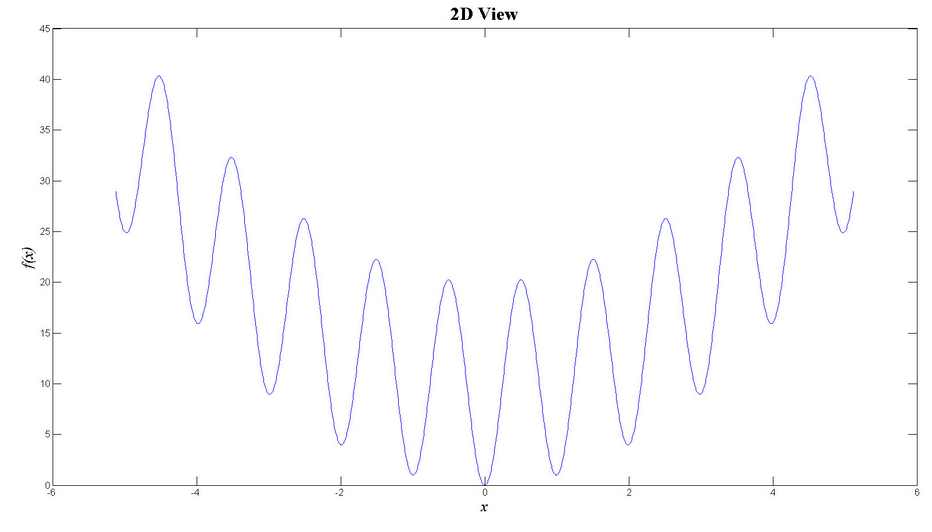
\includegraphics[width=0.8\textwidth]{rastrigin}
	\end{center}
	\hspace{1in}\parbox{4in}{\caption[Rastrigin-Funktion]{Rastrigin-Funktion}}
	\label{rastabb}
\end{figure}
\paragraph{Methode}
Das Modell zur Simulation der \acs{PSO} ist in dieser Arbeit als abstraktes Beispiel zur agentenbasierten Modellierung angeführt. Die Methode zum Finden des globalen Minimums der Rastrigin-Funktion stellt der im Kapitel 3.3 vorgestellte \acs{PSO}-Algorithmus dar.
\paragraph{Parameter}
Im Modell ist die Anzahl der Partikel, der Trägheitskoeffizient, der lokale Vertrauenskoeffizient und der globale Vertrauenskoeffizient einstellbar.
\newpage
\subsubsection{Futtersuche mit \acs{ACO} und \acs{PSO}}
\paragraph{Modellbeschreibung}
Im Modell der Futtersuche suchen die Agenten nach der Futterquelle in einer zweidimensionalen Agenten-Umgebung. Sie starten ihre Suche im Ameisenbau oder Bienenstock. Das erste Ziel des Modells ist das zufallsgesteuerte Finden der Futterquelle durch die Agenten. Im Anschluss interagieren die Agenten miteinander um die Futterquelle abzubauen. 
\paragraph{Methode\acs{ACO}}
Zum effizienten Abbau der Futterquelle kommunizieren die modellierten Ameisen über die zweidimensionale Agenten-Umgebung in Form von Pheromonmarkierungen. Im Modell gibt es zwei Pheromontypen die mit der Zeit verdunsten. Heimatpheromone markieren den Weg zum Ameisenbau und Futterpheromone den Weg zur Futterquelle. Auf der Suche nach der Futterquelle werden Heimatpheromone hinterlassen. Findet eine modellierte Ameise die Futterquelle wird eine Einheit der Futterquelle abgebaut. Nachdem die Futterquelle abgebaut wurde kehrt die Ameise zum Ameisenbau zurück. Dabei hinterlässt sie Futterpheromone. Befindet sich die modellierte Ameise im Ameisenbau liefert sie die Futtereinheit und begibt sich anschließend erneut auf Futtersuche. Der abgebildete Algorithmus \ref{futtersucheaco} fasst das Vorgehen für den Abbau der Futterquelle zusammen.
\begin{framed}
	\begin{algorithm}[H]
			\eIf{hatFuttereinheit}
			{
				Kehre zum Ameisenbau zurück (Folge Heimatpheromonen)\;
				Hinterlasse Futterpheromone\;
				\lIf{Position der Ameise == Position des Ameisenbaus}{
					hatFuttereinheit = false
				}
			}
			{
				Finde Futterquelle (Folge Futterpheromonen)\;
				Hinterlasse Heimatpheromone\;
				\lIf{Position der Ameise == Position der Futterquelle}{
					hatFuttereinheit = true
				}
			}
		\caption{Futtersuche mit \acs{ACO}}
		\label{futtersucheaco}
	\end{algorithm}
\end{framed}
\paragraph{Parameter \acs{ACO}}
Die einstellbaren Parameter des Modells sind die Anzahl der modellierten Ameisen und die in Kapitel 3.2.2 definierten Parameter $\alpha$ und $\beta$ der \acs{ACO}.
\paragraph{Methode \acs{BCO}}

\begin{framed}
	\begin{algorithm}[H]
		\eIf{InformationFutterquelle}
		{
			Bewege dich in die Richtung der Futterquelle\;
			Finde die Futterquelle\;
			Kehre zum Bienenstock zurück\;
			Tanze für aufgeschlossene Bienen\;
		}
		{
			\eIf{Tanzende Biene in der Umgebung}{
				Beobachte tanzende Bienen\;
				InformationFutterquelle = true\;
			}
			{
				Starte mit niedriger Wahrscheinlichkeit eine zufällige Suche nach der Futterquelle\;
				\eIf{Suchlimit}{
					Kehre zum Bienenstock zurück\;
				}
				{
					Finde die Futterquelle\;
					InformationFutterquelle = true\;
					Kehre zum Bienenstock zurück\;
					Tanze für aufgeschlossene Bienen\;					
				}	
			}
		}
		\caption{Futtersuche mit \acs{ACO}}
		\label{futtersuchebco}
	\end{algorithm}
\end{framed}
\paragraph{Parameter \acs{BCO}}

\newpage
\subsection{Framework}
\subsubsection{Anforderungen}
Die Anforderungen an das Framework zur Erstellung der in Kapitel 4.1 vorgestellten Modelle und anschließender grafischer Simulation sind:
\begin{itemize}
	\item \textbf{Open-Source + kostenlos:} Der Quelltext des Frameworks ist öffentlich. Zudem kann das Framework kostenlos genutzt werden.
	\item \textbf{Aktualität:} Es ist eine aktuelle und stabile Version des Frameworks verfügbar. 
	\item \textbf{Einsetzbarkeit:} Das Framework kann auf dem Betriebssystem Linux verwendet werden und unterstützt die Programmiersprache Java. Diese Anforderung entsteht durch die Präferenzen des Autors dieser Arbeit.
	\item \textbf{Visualisierung:} Modelle werden grafisch in 2D simuliert.
	\item \textbf{Dokumentation + Tutorial:} Das Framework ist umfangreich dokumentiert und besitzt ein Tutorial für Einsteiger.
	\item \textbf{Ausführungsgeschwindigkeit der Simulation:} Die Ausführungsgeschwindigkeit der Simulation ist hoch, trotz rechenintensiven Modellen mit vielen Agenten und Iterationen.
\end{itemize}
\subsubsection{Übersicht}
\paragraph{NetLogo}
NetLogo ist eine Open-Source-Plattform und wurde 1999 von U. Wilensky entwickelt. Die neuste Version 6.0.3 wurde im März 2018 veröffentlicht und steht für die Betriebssysteme Mac, Windows und Linux zur Verfügung. Die proprietäre funktionale Programmiersprache und die ausführliche Dokumentation machen es Einsteigern ohne Programmierkenntnisse einfach erste eigene Modelle zu implementieren. Das Fehlen objektorientierter Features schränkt die Funktionalität und Erweiterbarkeit des Frameworks jedoch ein. Darüber hinaus verfügt NetLogo über keine explizite Unterstützung für die Trennung zwischen Agenten, Agenten-Beziehungen und Agenten-Umgebung.
\paragraph{Mason}
Mason ist eine Java-Bibliothek, die ein breitgefächertes Repertoire an Funktionen für die \acs{ABM} bereitstellt. Die aktuelle Version 1.9 wurde im Juni 2015 veröffentlicht. Eine umfangreiche Dokumentation der Open-Source-Bibliothek und ein einsteigerfreundliches Tutorial erlauben es innerhalb weniger Stunden eine erste lauffähige Simulation zu erstellen. Kombiniert mit der JFreeChart-Bibliothek ist es zudem möglich die Simulationen in grafischer Form auszuwerten.
\paragraph{Swarm}
Swarm ist eine der ersten \acs{ABM}-Plattformen. Ursprünglich wurde Swarm 1997 am Santa Fe Institute entwickelt und veröffentlicht. Die ABM-Plattform Swarm war zuerst nur auf UNIX-basierten Betriebssystemen einsetzbar und unterstützte nur die Programmiersprache Objective-C. Heute steht Swarm für die Betriebssysteme Mac, Windows und Linux zur Verfügung und unterstützt neben Objective-C auch Java. Das Framework ist Open-Source. Version 2.4.1 wurde im April 2009 veröffentlicht.
\paragraph{Repast}
Repast ist eine Open-Source-Plattform für die \acs{ABM} und Simulation. Die Software ist für die Betriebssysteme Mac, Windows und Linux verfügbar. Es existieren zwei verschiedene Editionen der Plattform. Repast Simphony implementiert grundlegende und erweiterte Konzepte der \acs{ABM}. Unterstützt werden die Programmiersprachen Java, Logo und Groovy. Repast High Performance Computing ist ein agentenbasiertes Modellierungssystem speziell entwickelt für die parallele Ausführung der Simulationen auf verteilten Systemen. Zur Modellentwicklung mit dieser Edition von Repast werden umfangreiche Programmierkenntnisse in C++ vorausgesetzt. Die stabile Version 2.5 von Repast Symphonie wurde im Oktober 2017 veröffentlicht. 
\paragraph{Zusammenfassung}
S.F. Railsback, S.L. Lytinen und S.K. Jackson untersuchten im Jahr 2006 verschiedene Plattformen für die \acs{ABM} und Simulation. Ihre Ergebnisse über die oben genannten \acs{ABM}-Plattformen können folgendermaßen zusammengefasst werden:
\begin{itemize}
	\item \textbf{NetLogo:} Netlogo ist einfach zu bedienen und besitzt eine umfangreiche Dokumentation. NetLogo ist eine gute Wahl für simple Modelle bei denen die Ausführungszeit der Simulation eine untergeordnete Rolle spielt. Außerdem eignet sich NetLogo zur Erstellung eines Modellprototyps. Dieser Prototyp kann anschließend in anderen \acs{ABM}-Plattformen erweitert werden.
	\item \textbf{Mason:} Mason ist eine gute Wahl für erfahrene Programmierer, die an rechenintensiven Modellen mit vielen Agenten und Iterationen arbeiten. Ein Vorteil von Mason ist die Reproduzierbarkeit der Simulationsergebnisse auf verschiedenen Betriebssystemen.
	\item \textbf{Swarm:} Swarm ist stabil, klein, gut organisiert und unterstützt komplexe Modelle. Voraussetzung für einen schnellen Einstieg ist Programmiererfahrung mit Objective-C.
	\item \textbf{Repast:} Repast ist die vollständigste \acs{ABM}-Plattform und hat eine vergleichsweise schnelle Ausführungszeit der Simulationen. Die Dokumentation ist teilweise unvollständig.
\end{itemize}
\subsubsection{Auswahl}
Tabelle \ref{tabframework} zeigt eine Übersicht der Frameworks und die erfüllten Anforderungen.
Zur Implementierung der in Kapitel 4.1 beschriebenen Modelle wird Mason als Framework gewählt. Mit Mason können die Modelle in Java implementiert werden. Da im Zuge dieser Studienarbeit rechenintensive Simulationen mit vielen Agenten durchgeführt werden sollen ist die hohe Ausführungsgeschwindigkeit der Simulationen wichtig. Mason bietet zudem eine umfangreiche Dokumentation und sowie ein 14-stufiges Tutorial. 
\begin{table}[h]
	\begin{tabular}{p{1.5cm}|p{1.5cm}|p{1.6cm}|p{1.7cm}|p{1.3cm}|p{1.3cm}|p{2.7cm}}
		& Open-Source + kostenlos & Aktuali-tät & Einsetz-barkeit & Visuali-sierung & Doku + Tutorial & Geschwindig-keit\\ \hline\hline
		NetLogo & $\surd$ & Mrz. 2018 & $X$ & 2D/3D & $\surd$ & langsam\\ \hline
		Mason & $\surd$ & Jun. 2015 & $\surd$ & 2D/3D & $\surd$ & sehr schnell\\ \hline
		Swarm & $\surd$  & Apr. 2009 & $\surd$ & 2D/3D & $X$ & langsam\\ \hline
		Repast & $\surd$ & Okt. 2017 & $\surd$ & 2D/3D & $\surd$ & schnell\\ \hline
	\end{tabular}
	\caption{Auswahl des Frameworks}
	\label{tabframework}
\end{table}
\newpage
\section{Implementierung}
\subsection{Mason}

\subsection{Finden des globalen Minimums einer Funktion mit \acs{PSO}}
Bei der Implementierung des Modells wird ein Großteil der Funktionen des Modells von A. Desai, S. Luke und G. Mason verwendet. Ihr Modell darf modifiziert und veröffentlicht werden. Um die Implementierung des in Kapitel 4.1.1 definierten Modells zu beschreiben wird die Implementierung anhand der Schritte des \acs{PSO}-Algorithmus aus Kapitel 3.1.3 beschrieben.
\subsubsection{Initalisiere Partikelschwarm im Suchraum}
\begin{lstlisting}[caption= xxxxxxx,label = xxxx]
public void start(){
	bestVal = 0;
	super.start();
	particles = new Particle[numParticles];
	space = new Continuous2D(height, width, height);
	Evaluatable f = mapFitnessFunction(fitnessFunction);            
	//Initalisiere Partikel
	for (int i = 0; i < numParticles; i++){
		double x = (random.nextDouble() * width) - (width * 0.5);
		double y = (random.nextDouble() * height) - (height * 0.5);
		double vx = (random.nextDouble() * initialVelocityRange) - (initialVelocityRange * 0.5);
		double vy = (random.nextDouble() * initialVelocityRange) - (initialVelocityRange * 0.5);

		final Particle p = new Particle(x, y, vx, vy, this, f, i);
		particles[i] = p;
	}
}
\end{lstlisting}
\subsubsection{Bestimme Position und Geschwindigkeit}
\begin{lstlisting}[caption= xxxxxxx,label = xxxx]
public Particle(double x, double y, double vx, double vy, PSO pso, Evaluatable f) {
	super();
	//Bestimme Position und Geschwindigkeit der Partikel
	this.position.setTo(x, y);
	this.velocity.setTo(vx, vy);

	this.pso = pso;
	this.fitnessFunction = f;
	pso.space.setObjectLocation(this,new Double2D(position));
}
\end{lstlisting}
\subsubsection{Bestimme den Fitnesswert}
\begin{lstlisting}[caption= xxxxxxx,label = xxxx]
public class Rastrigin implements Evaluatable{
	private static final long serialVersionUID = 1;

	public double calcFitness(double x, double y){
		return (1000 - (20 + x*x - 10*Math.cos(2*Math.PI*x) + y*y - 10*Math.cos(2*Math.PI*y)));
	}
}
\end{lstlisting}
\subsubsection{Bestimme beste Position} 
\begin{lstlisting}[caption= xxxxxxx,label = xxxx]
public void updateBest(double currVal, double currX, double currY){
	if (currVal > bestVal){
		bestVal = currVal;
		bestPosition.setTo(currX, currY);
		pso.updateBest(currVal, currX, currY);
	}
}
\end{lstlisting}
\subsubsection{Berechne neue Position}
\begin{lstlisting}[caption= xxxxxxx,label = xxxx]
public void stepUpdatePosition(){
	position.addIn(velocity);
	pso.space.setObjectLocation(this, new Double2D(position));
}
//Defintion von addIn
public final MutableDouble2D addIn(final MutableDouble2D other){
	x = other.x + x;
	y = other.y + y;
	return this;
}
\end{lstlisting}
\subsubsection{Berechne neue Geschwindigkeit}
\begin{lstlisting}[caption= xxxxxxx,label = xxxx]
public void stepUpdateVelocity(){

	double x = position.x;
	double y = position.y;
	double inertia = velocity.x;
	double pDelta = bestPosition.x - x;
	double gDelta = pso.bestPosition.x - x;
	double pWeight = Math.random() + 0.4;
	double gWeight = Math.random() + 0.4;
	double vx = (0.9*inertia + pWeight*pDelta + gWeight*gDelta) / (1+pWeight+nWeight+gWeight);

	inertia = velocity.y;
	pDelta = bestPosition.y - y;
	gDelta = pso.bestPosition.y - y;
	pWeight = Math.random() + 0.4;
	gWeight = Math.random() + 0.4;
	double vy = (0.9*inertia + pWeight*pDelta + gWeight*gDelta) / (1+pWeight+nWeight+gWeight);

	velocity.setTo(vx, vy);         
} 
\end{lstlisting}
\subsection{Futtersuche mit \acs{ACO}}

\subsection{Futtersuche mit \acs{BCO}}
\section{Experimente}
\section{Zusammenfassung}

\newpage
\begin{thebibliography}{sotief}
	\bibitem{1}A. Aulinger. Kollektive Intelligenz: Methoden, Erfahrungen und Perspektiven. Entstehungsjahr: 2009.
	\bibitem{2}M. Dorigo, V. Maniezzo, A. Colorni. Ant System: An Autocatalytic Optimizing Process. Technical Report 91-016 Revised.  Entstehungsjahr: 1991.
	\bibitem{6}Y. Liu. Partikelschwarmoptimierung für diskrete Probleme. Technische Universität München. Entstehungsjahr: 2014.\newline\newline
	Weblink: http://lydiapintscher.de/uni/schwarmintelligenz.pdf \newline Einsichtnahme: 14.01.2018
	\bibitem{2}C. Macal, M. North. Tutorial on agent-based modelling and simulation. Journal of Simulation 4, Nr. 1, Seite 151-162. Entstehungsjahr: 2010.
	\bibitem{3}L. Pintscher. Schwarmintelligenz. Universität Karlsruhe. Entstehungsjahr: ohne Jahr.\newline\newline
	Weblink: http://lydiapintscher.de/uni/schwarmintelligenz.pdf \newline Einsichtnahme: 14.01.2018
	\bibitem{4}S. Russel, P. Norvig. Artificial Intelligence: A Modern Approach. Upper Saddle River. Entstehungsjahr: 2009.
	\bibitem{1}W.M. Wheeler. The Ant Colony as an Organism. Journal of Morphology Volume 22, Issue 2, Seite 307-325. Entstehungsjahr: 1911.\newline\newline
	Weblink: http://www3.interscience.wiley.com/journal/109914213/abstract \newline Einsichtnahme: 04.01.2018
	\bibitem{5}M. Wooldridge, N. Jennings. Intelligent Agents: Theory and Practice. Knowledge Engineering Review 10, Nr. 2, Seite 115-152. Entstehungsjahr: 1995.

	
\end{thebibliography}
\newpage
%\appendix
\appendixtoc
\newpage
\section{Anhang}
\subsection{Quellcode Futtersuche mit \acs{ACO}}
\subsubsection{Kehre zum Ameisenbau zurück + (Folge Heimatpheromonen)}
\begin{lstlisting}[caption= xxxxxxx,label = xxxx]
double max = AntsForage.IMPOSSIBLY_BAD_PHEROMONE;

int max_x = x;
int max_y = y;
int count = 2;

for(int dx = -1; dx < 2; dx++) {
for(int dy = -1; dy < 2; dy++) {

int _x = dx+x;
int _y = dy+y;

if ((dx == 0 && dy == 0) || _x < 0 || _y < 0 || _x >= AntsForage.GRID_WIDTH || _y >= AntsForage.GRID_HEIGHT ||  af.obstacles.field[_x][_y] == 1) continue;

double m = af.toHomeGrid.field[_x][_y];


if (m > max) {count = 2;}

if (m > max || (m == max && state.random.nextBoolean(1.0 / count++))) {
max = m;
max_x = _x;
max_y = _y;
}
}
}

if (max == 0 && last != null) {

if (state.random.nextBoolean(af.momentumProbability)) {
int xm = x + (x - last.x);
int ym = y + (y - last.y);

if (xm >= 0 && xm < AntsForage.GRID_WIDTH && ym >= 0 && ym < AntsForage.GRID_HEIGHT && af.obstacles.field[xm][ym] == 0) { 
max_x = xm; 
max_y = ym; 
}
}
} else if (state.random.nextBoolean(af.randomActionProbability)) {
int xd = (state.random.nextInt(3) - 1);
int yd = (state.random.nextInt(3) - 1);
int xm = x + xd;
int ym = y + yd;

if (!(xd == 0 && yd == 0) && xm >= 0 && xm < AntsForage.GRID_WIDTH && ym >= 0 && ym < AntsForage.GRID_HEIGHT && af.obstacles.field[xm][ym] == 0) { 
max_x = xm; 
max_y = ym; 
}
}

af.buggrid.setObjectLocation(this, new Int2D(max_x, max_y));

if (af.sites.field[max_x][max_y] == AntsForage.HOME) { 
hasFoodItem = ! hasFoodItem; 
}
\end{lstlisting}
\end{document}


